\section{Study 4: automated facial analysis}
\label{s:study4}

This study presents a method for automated analysis of facial cues from videos with an empirical evaluation of its application as a potential tool for detecting stress and boredom of players. The proposed automated facial analysis is based on the measurement of 7 facial features ($F_1$ to $F_7$) calculated from 68 detected facial landmarks. Facial features are mainly based on the Euclidean distance of landmarks and they do not rely on pre-defined expressions, i.e. 6 universal facial expressions, nor training of a model nor the use of standards related to the face, e.g. MPEG4 and FACS. Additionally, the method does not use an arbitrarily selected frame as a reference for calculations since features are derived from each frame (or a small set of past frames). Features are obtained unobtrusively via computer vision analysis focused on detecting the activity of facial muscles reported by previous work involving emotion detection in games.

%This study introduces a method for automated analysis of facial cues from videos, presenting empirical results of its application as a potential tool for detecting stress and boredom of players in games. The method is based on Euclidean distances between automatically detected facial points, not relying on prior model training to produce results. Additionally the method is able to cope with face analysis under challenging conditions, such as when players behave naturally, e.g. moving and laughing while playing games. The method was applied on the video recordings to contextualize the automated facial analysis in a more game-oriented fashion than previous work.

%%%%%%%%%%%%%%%%%%%%%%%%%%%%%%%%%%%%%%%%%%%%%%%%%%%%%%%%%%%%%%%%%%%%%%%%%%%%%%%%%%%%%
\subsection{Facial features}
\label{s:experiment1-study4-features-extraction}

The automated facial analysis we propose is based on the measurement of 7 facial features calculated from 68 detected facial landmarks. Table \ref{table:features} presents the facial features, which are illustrated in Figure \ref{fig:faces}(b). Our facial features are mainly based on the Euclidean distances between landmarks, similarly to some works previously mentioned, however our approach does not rely on pre-defined expressions, i.e. 6 universal facial expressions, training of a model, or the use of the MPEG-4 standard, which specifies representations for 3D facial animations, not emotional interactions in games. Additionally our method does not use an arbitrarily selected frame, e.g. the 100\textsuperscript{th} frame \cite{giannakakis2017stress}, as a reference for calculations, since our features are derived from each frame (or a small set of past frames). Our features are obtained unobtrusively via computer vision analysis focused on detecting activity of facial muscles reported by previous work involving EMG and emotion detection in games. We believe our approach is more user-tailored, convenient and better suited for contexts involving games.

The process of extracting our facial features has two main steps: face detection and feature calculation. In the first step, computer vision techniques are applied to a frame of the video and facial landmarks are detected. In the second step, the detected landmarks are used to calculate several facial features related to eyes, mouth, and head movement. The following sections present in detail how each step is performed, including details regarding the calculation of features.

% zygomatic -> smiling
% orbicularis oculi -> eyelid control
% corrugator -> frowning

\begin{landscape}
\begin{table*}
    \centering
    \caption{Information regarding calculated facial features}
    \label{table:features}
    \begin{tabular}[l]{@{}lcp{11cm}}
        \hline
            \textbf{Name} & \textbf{Notation} & \textbf{Description} \\
        \hline
            Mouth outer & $F_1$ & Sum of the Euclidean distance between the mouth contour landmarks and the anchor landmarks. It monitors the zygomatic muscle.  \\
            Mouth corner & $F_2$ & Sum of the Euclidean distance between the mouth corner landmarks and the anchor landmarks. It monitors the zygomatic muscle. \\
            Eye area & $F_3$ & Area of the regions bounded by the closed curves formed by the landmarks in contour of the eyes. It monitors the orbicularis oculi muscle. \\
            Eyebrow activity & $F_4$ & Sum of the Euclidean distance between eyebrow landmarks and the anchor landmarks. It monitors the corrugator muscle.  \\
            Face area & $F_5$ & Area of the region bounded by the closed polygon formed by the most external detected landmarks.  \\
            Face motion & $F_6$ & Average value of the Euclidean norm of a set of landmarks in the last $N$ frames. It describes the total distance the head has moved in any direction in a short period of time.  \\
            Facial COM & $F_7$ & Average value of all detected landmarks. It describes the overall movement of all facial landmarks.  \\
        \hline
    \end{tabular}
\end{table*}
\end{landscape}

%%%%%%%%%%%%%%%%%%%%%%%%%%%%%%%%%%%%%%%%%%%%%%%%%%%%%%%%%%%%%%%%
\subsubsection{Face detection}

The face detection procedure is performed for every frame of the input video. We detect the face using a Constrained Local Neural Field (CLNF) model \cite{baltrusaitis2013constrained,baltruvsaitis2016openface}. CLNF uses a local neural field patch expert that learns the nonlinearities and spatial relationships between pixel values and the probability of landmark alignment. The technique also uses a non-uniform regularized landmark Mean Shift fitting technique that takes into consideration patch reliabilities. It improves the detection process under challenging conditions, e.g. extreme face pose or occlusion, which is likely to happen in game sessions \cite{bevilacqua2016variations}. The application of the CLNF model to a given video frame produces a vector $L$ of 68 facial landmarks:

\[
L = [p_0, p_1, p_2, \dots, p_{67}]^T
\]

where $p_i$ is a detected facial landmark that represents a 2D coordinate $(x_i, y_i)$ in the frame. Facial landmarks are related to different facial regions, such as eyebrows, eyes and lips. Figure \ref{fig:faces}(a) illustrates the landmarks of $L$ in a given frame.

\begin{figure}
\centering
  \begin{subfigure}[b]{0.5\textwidth}
    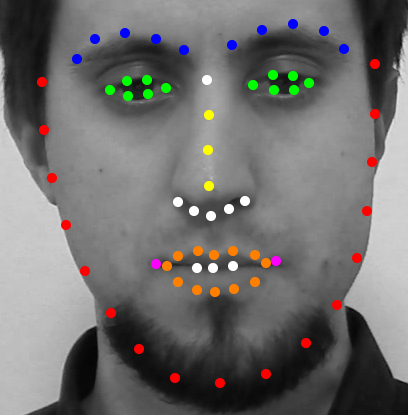
\includegraphics[width=0.95\textwidth]{figures/facial-landmarks-detail.png}
    \caption{}
    \label{fig:face-occlusion}
  \end{subfigure}%
  \begin{subfigure}[b]{0.5\textwidth}
    \centering
    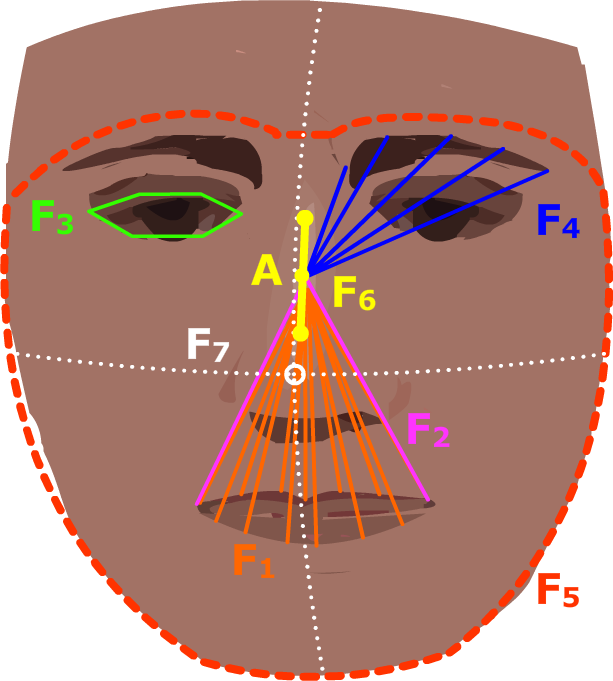
\includegraphics[width=0.95\textwidth]{figures/facial-features.png}
    \caption{}
    \label{fig:head-tilt}
  \end{subfigure}
  \caption{Facial landmarks and features. (a) Highlight of 68 detected facial landmarks. (b) Visual representation of our facial features.}
  \label{fig:faces}
\end{figure}


%%%%%%%%%%%%%%%%%%%%%%%%%%%%%%%%%%%%%%%%%%%%%%%%%%%%%%%%%%%%%%%%
\subsubsection{Anchor landmarks}

The calculation of our facial features involves the Euclidean distance among facial landmarks. Subsequently the Euclidean distance between two landmarks $a_1 = (x_1, y_1)$ and $a_2 = (x_2, y_2)$ is given as:

\[
d(a_1,a_2) = \sqrt{(x_2 - x_1)^2 + (y_2 - y_1)^2}
\]

Landmarks in the nose area are more likely to be stable, presenting fewer position variations in consecutive frames \cite{giannakakis2017stress}. Consequently they are good reference points to be used in the calculation of the Euclidean distance among landmarks. In order to provide stable reference points for the calculation of our facial features, we selected 3 highly stable landmarks located in the nose line, denoted as the anchor vector $A = [p_{28}, p_{29}, p_{30}]^T$. The landmarks of the anchor vector $A$ are highlighted in yellow in Figure \ref{fig:faces}(a).

%%%%%%%%%%%%%%%%%%%%%%%%%%%%%%%%%%%%%%%%%%%%%%%%%%%%%%%%%%%%%%%%
\subsubsection{Feature normalization}

Subjects moved towards and away from the camera during the gaming sessions. This movement affects the Euclidean distance between landmarks, as it tends to increase when the subject is closer to the camera, for instance. Additionally subjects have unique facial shapes and characteristics, which also affect the calculation and comparison of the facial features between subjects. To mitigate that problem, we calculated a normalization coefficient $K$ as the Euclidean distance between the upper and lower most anchor landmarks in $A$. In other words, $K$ represents the size of the subjects nose line. Since all features are divided by $K$, their final value is expressed as normalized pixels (relative to $K$) rather than pixels \textit{per se}.

%%%%%%%%%%%%%%%%%%%%%%%%%%%%%%%%%%%%%%%%%%%%%%%%%%%%%%%%%%%%%%%%
\subsubsection{Mouth related features}

Mouth related features aim to detect activity in the zygomatic muscles, illustrated in Figure \ref{fig:face-muscles} (c and d, page \pageref{fig:face-muscles}), which are related to changes in the mouth, such as lips activity (stretch, suck, press, parted, tongue touching, bite) and movement (including talking). We calculate two facial features related to the mouth area: mouth outer and mouth corner.

\paragraph{Mouth outer ($F_1$):} given vector $M = [p_{48}, p_{49}, \dots, p_{60}]^T$ containing the landmarks in the outer part of the mouth (highlighted in orange in Figure \ref{fig:faces}(a)). The mouth outer feature is calculated as the sum of the Euclidean distance among the landmarks in $M$ and the anchor landmarks in $A$:

\[
F_1 = \frac{1}{K} \sum_{i=1}^{12} \sum_{j=1}^{3} d(A_j, M_i)
\]

where $A_j$ and $M_i$ are the $j$-th and $i$-th element of $A$ and $M$, respectively.

\paragraph{Mouth corner ($F_2$):} given vector $C = [p_{48}, p_{54}]^T$, containing the two landmarks representing the mouth corners (highlighted in pink in Figure \ref{fig:faces}(a)). The mouth corner feature is the sum of the Euclidean distance among the landmarks in $C$ and $A$:

\[
F_2 = \frac{1}{K} \sum_{i=1}^{2} \sum_{j=1}^{3} d(A_j, C_i)
\]

where $A_j$ and $C_i$ are the $j$-th and $i$-th element of $A$ and $C$, respectively.

%%%%%%%%%%%%%%%%%%%%%%%%%%%%%%%%%%%%%%%%%%%%%%%%%%%%%%%%%%%%%%%%
\subsubsection{Eye related features}

Eye related features aim to detect activity related to the orbicularis oculi and the corrugator muscles, illustrated in Figure \ref{fig:face-muscles}(b) and Figure \ref{fig:face-muscles}(a) respectively, which comprehend changes in the eyes region, including eye and eyebrow activity. We calculated two facial features related to the eyes: eye area and eyebrow activity.

\paragraph{Eye area ($F_3$):} given vector $Y_l = [p_{36}, p_{37}, \dots, p_{41}]^T$ containing the landmarks describing the left eye, highlighted in green in Figure \ref{fig:faces}(a), and vector $Y_r = [p_{42}, p_{43}, \dots, p_{47}]^T$ containing the landmarks describing the right eye, highlighted in green in Figure \ref{fig:faces}(a). The eye area feature is the area of the regions bounded by the closed curves formed by the landmarks in $Y_l$ and $Y_r$, divided by $K$. We calculated the area of the curves using OpenCV's \texttt{contourArea()} function, which uses Green's theorem \cite{stewart2011calculus}.

\paragraph{Eyebrow activity ($F_4$):} calculated as the sum of the Euclidean distances among the eyebrow landmarks and the anchor landmarks in $A$. Given the vector $W_l = [p_{17}, p_{18}, \dots, p_{21}]^T$ containing the landmarks describing the left eyebrow, highlighted in blue in Figure \ref{fig:faces}(a), and the set $W_r = [p_{22}, p_{23}, \dots, p_{26}]^T$ containing the landmarks describing the right eyebrow, highlighted in blue in Figure \ref{fig:faces}(a). The eyebrow activity feature is calculated as:

\[
F_4 = \frac{1}{K} \sum_{i=1}^{5} \sum_{j=1}^{3} \Big[ d(A_j, W_{l,i}) + d(A_j, W_{r,i}) \Big]
\]

where $A_j$, $W_{l,i}$ and $W_{r,i}$ are the $j$-th, $i$-th and $i$-th element of $A$, $W_l$ and $W_r$, respectively.

%%%%%%%%%%%%%%%%%%%%%%%%%%%%%%%%%%%%%%%%%%%%%%%%%%%%%%%%%%%%%%%%
\subsubsection{Head related features}

Head related features aim to detect body movements, in particular variations of head pose and amount of motion the head/face is performing over time. We calculated three features related to the head: face area, face motion and facial center of mass (COM).

\paragraph{Face area ($F_5$):} during the interaction with a game, subjects tend to move towards (or away from) the screen, which causes the facial area in the video recordings to increase or decrease. Given vector $F = [p_{0}, p_{1}, \dots, p_{16}]^T$ containing the landmarks describing the contour of the face, highlighted in red in Figure \ref{fig:faces}(a). The face area feature is the area of the region bounded by the closed curves formed by the landmarks in $F \cup W_r \cup W_l$, divided by $K$. Similarly to the eye area, we calculated the area under the curves using OpenCV's \texttt{contourArea()} function.

\paragraph{Face motion ($F_6$):} accounts for the total distance the head has moved in any direction in a short period of time. For each frame of the video, we save the currently detected anchor vector $A$, which produces vector $D = [A_1, A_2, \dots, A_n]^T$, where $A_i$ is the vector $A$ detected in the $i$-th frame of the video and $n$ is number of frames in the video. We then calculate the face motion feature as:

\[
F_6 = \frac{1}{K} \sum_{j=1}^{3} \sum_{t=1}^{Z - 1} || D(f - t, j) - D(f - Z, j) ||
\]

where $Z$ is the amount of frames to include in the motion analysis, $D(i,j)$ is the $j$-th element of $A_i \in D$, $f$ is the number of the current frame, and $||.||$ is the Euclidean norm. In our analysis, we used $Z=50$ (50 frames, equivalent to 1 second).

\paragraph{Facial COM ($F_7$):} describes the overall movement of all facial landmarks. A single 2D point, calculated as the average of all landmarks in $L$, is used to monitor the movement. The COM feature is calculated as:

\[
F_7 = \frac{1}{K} \frac{1}{N} \sum_{i=1}^{N} || p_i ||
\]

where $N$ is the total number of detected landmarks (elements in $L$) and $||.||$ is the Euclidean norm.

%%%%%%%%%%%%%%%%%%%%%%%%%%%%%%%%%%%%%%%%%%%%%%%%%%%%%%%%%%%%%%%%
\subsection{Analysis and methods}
\label{s:experiment1-study4-feature-analysis}

%%%%%%%%%%%%%%%%%%%%%%%%%%%%%%%%%%%%%%%%%%%%%%%%%%%%%%%%%%%%%%%%
\subsubsection{Data pre-processing}

The pre-processing of video recordings involved extraction of the parts containing the interaction with the games and the discard of noisy frames. Firstly we extracted from the video recordings the periods where subjects were playing each one of the available games. It resulted in three videos per subject, denoted as $V_{s,i}$ where $s$ is the $s$-th subject and $i \in \{1, 2, 3\}$ represents the game.

\begin{figure}
\centering
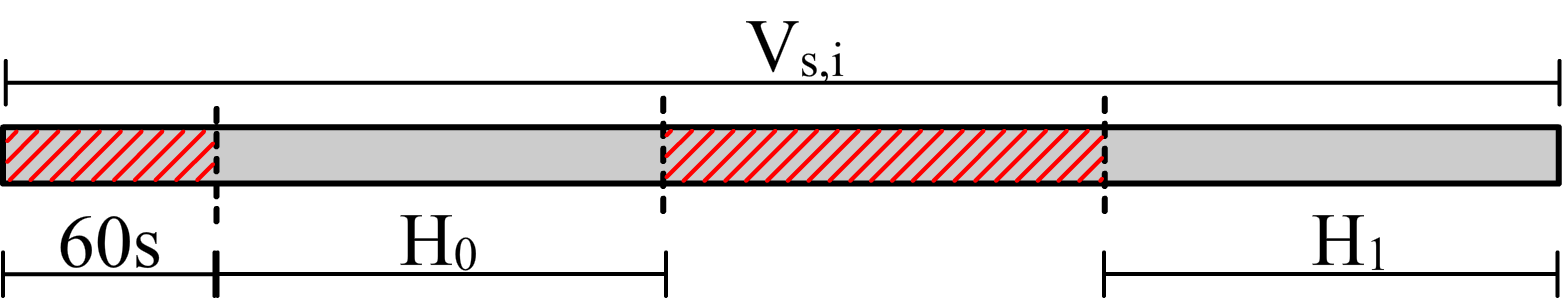
\includegraphics[width=0.9\textwidth]{figures/pre-processing}
\caption{Extraction of video segments $H_0$ and $H_1$ containing boring and stressful game interactions, respectively. Initial 60 seconds of any video $V_{s,i}$ are ignored and the remaining is divided into three pieces, from which the first and the last ones are selected. Stripes highlight discarded video segments.}
\label{fig:preprocessing}
\end{figure}

As previously mentioned, the games used as emotional elicitation material in the experiment induced variations of physiological signals on subjects, who perceived them as being boring at the beginning and stressful at the end. Since our aim is to test the potential of our facial features to differentiate emotional states of boredom and stress, we extracted from each video $V_{s,i}$ two video segments, named $H_0$ and $H_1$, whose subject's emotional state is assumed to be known and related to boredom and stress. In order to achieve that, we performed the following extraction procedure, illustrated in Figure \ref{fig:preprocessing}. Firstly we ignored the initial 60 seconds of any given video $V_{s,i}$. The remaining of the video was then divided into three pieces, from which the first and the last were selected as $H_0$ and $H_1$, respectively.

The reason why we discarded the initial part of all game videos is because we believe the first minute might not be ideal for a fair analysis. During the first minute of gameplay, subjects are less likely to be in their usual neutral emotional state. They are more likely to be stimulated by the excitement of the initial contact with a game soon to be played, which interferes with any feelings of boredom. Additionally subjects need basic experimentation with the game to learn how to play it and judge if it is boring or not. Such claim is supported by empirical analysis of the first minute of the video recordings that show repeated head and eye movements from and towards the keyboard/display. As per our understanding, the second minute and onward in the videos is more likely to portrait facial activity related to emotional reactions to the game instead of facial activity connected to gameplay learning. Regarding the division of the remaining part of the video into three segments, from which two were selected as $H_0$ and $H_1$, we followed the reasoning that the emotional state of subjects was unknown in the middle part of $V_{s,i}$. Based on self-reported emotional states, subjects reported the beginning part of the games as boring and the final part as stressful; additionally there are significant differences in the HR mean between the second and the last minute of gameplay in the games \cite{bevilacqua2018changes}. Consequentially we understand that video segments $H_0$ and $H_1$ accurately portray interaction of subjects during boring and stressful periods of the games, respectively.

The pre-processing of the recordings resulted in 6 video segments per subjects: 3 segments $H_0$ (one per game) and 3 segments $H_1$ (one per game). A given game $i$ contains $N=20$ pairs of $H_0$ and $H_1$ video segments (20 segments $H_0$, one per subject, and 20 segments $H_1$, one per subject). When considering all subjects and games, there are $N=60$ pairs of $H_0$ and $H_1$ video segments (3 games $\times$ 20 subjects, resulting in 60 segments $H_0$ and 60 segments $H_1$). Subject 9 had problems playing the Platformer game, so segments $H_0$ and $H_1$ from subject 9 in the Platformer game were discarded. Consequentially the Platformer game contains $N=19$ pairs of $H_0$ and $H_1$ video segments; regarding all games and subjects, there are $N=59$ pairs of $H_0$ and $H_1$ video segments.

%%%%%%%%%%%%%%%%%%%%%%%%%%%%%%%%%%%%%%%%%%%%%%%%%%%%%%%%%%%%%%%%
\subsubsection{Feature analysis}

The previously mentioned features can be calculated for each frame of any given video, however facial cues might be better contextualized if analyzed in multiple frames. For that reason, we applied our facial analysis to all frames of all video segments $H_0$ and $H_1$. We then calculated the mean value of each facial feature in each video segment. As a result, any facial feature $F_i$ has $N=59$ pairs of mean values (59 from $H_0$ and 59 from $H_1$). From now on, we will refer to the set of mean values in $H_0$ or $H_1$ of a given feature $F_i$ simply as feature value in $H_0$ or $H_1$, respectively.
%Each mean value was calculated from all frames of a video segment ($H_0$ or $H_1$) of a subject in a particular game.

Based on a previous manual analysis of facial actions of the video recordings \cite{bevilacqua2016variations} and findings of related work, values of facial features during boring periods of the games are expected to be different than those during stressful periods. Since subjects perceived the games as boring at the beginning and stressful at the end, we assume that values in $H_0$ and $H_1$, for all features, are likely to correlate with an emotional state of boredom and stress, respectively. Consequentially we state the following overarching hypothesis: the mean value of features in $H_0$ is different than the mean value in $H_1$, for all subjects and games. More specifically, we can describe the overarching hypothesis as 7 sub-hypotheses, denoted $u_i$, where $i \in \{1, 2, ..., 7\}$. Hypothesis $u_i$ states that the true difference in means between the value of a given feature $F_i$ in $H_0$ and $H_1$, for all subjects, is greater than zero. The dependent variable of $u_i$ is $F_i$ and the null hypothesis is that the true difference in means between $H_0$ and $H_1$ for feature $F_i$, for all subjects and games, is equal to zero.

We tested hypothesis $u_i$ by performing a paired two-tail t-test on the values $H_0$ and $H_1$ of feature $F_i$. We performed 7 tests in total: $u_1$ (mouth outer), $u_2$ (mouth corner), $u_3$ (eye area), $u_4$ (eyebrow activity), $u_5$ (face area), $u_6$ (face motion), and $u_7$ (facial COM).

%%%%%%%%%%%%%%%%%%%%%%%%%%%%%%%%%%%%%%%%%%%%%%%%%%%%%%%%%%%%%%%%%%%%%%%%%%%%%%%%%%%%%
\subsection{Results}
%%%%%%%%%%%%%%%%%%%%%%%%%%%%%%%%%%%%%%%%%%%%%%%%%%%%%%%%%%%%%%%%%%%%%%%%%%%%%%%%%%%%%

Table \ref{table:changes} presents the mean of differences of all features between periods $H_0$ and $H_1$, calculated for all subjects in all games according to the description in Section \ref{s:experiment1-study4-features-extraction} and analyzed according to the procedures described in Section \ref{s:s:experiment1-study4-feature-analysis}. The mean of differences of all features show a decrease from $H_0$ to $H_1$. Comparing the mean difference of a feature to its mean value in $H_0$, the decrease from $H_0$ to $H_1$ was 10.7\% for mouth outer ($F_1$), 11.8\% for mouth corner ($F_2$), 10.4\% for eye area ($F_3$), 8.1\% for eyebrow activity ($F_4$), 9.4\% for face area ($F_5$), 8.2\% for face motion ($F_6$), and 11\% for facial COM ($F_7$). Changes related to $F_6$ and $F_7$ were not statistically significant. All remaining features presented statistically significant changes from $H_0$ to $H_1$. The highest decrease with statistical significance was associated with mouth corner, followed by mouth outer, eye area, face area, and eyebrow activity. Those numbers support our experimental expectations that the values for facial features are different when compared between two distinct parts of the games, i.e. boring and stressful ones.

\begin{table}
    \caption{Mean of differences ($\pm$SD) of features between periods $H_0$ and $H_1$ ($N=59$). Units expressed in normalized pixels.}
    \label{table:changes}
    \centering
    \begin{threeparttable}
        \begin{tabular}{lc}
            \hline
                \textbf{Feature (notation)} &  \\
            \hline
                Mouth outer ($F_1$)      & -20.59 $\pm$ 57.36\textsuperscript{**} \\
                Mouth corner ($F_2$)     & -3.90 $\pm$ 10.16\textsuperscript{**} \\
            \hline
                Eye area ($F_3$)         & -0.019 $\pm$ 0.064\textsuperscript{*} \\
                Eyebrow activity ($F_4$) & -15.59 $\pm$ 49.71\textsuperscript{*} \\
            \hline
                Face area ($F_5$)        & -2.60 $\pm$ 7.90\textsuperscript{*} \\
                Face motion ($F_6$)      & -44.97 $\pm$ 326.74 \\
                Facial COM ($F_7$)       & -0.029 $\pm$ 0.113 \\
            \hline
        \end{tabular}
        \begin{tablenotes}
          \small
          \item[*]{$p < 0.05$}
          \item[**]{$p < 0.01$}
        \end{tablenotes}
    \end{threeparttable}
\end{table}

The two facial features related to mouth, i.e. mouth corner and mouth outer, presented a combined average decrease of 11.24\% from $H_0$ to $H_1$. The change was the highest compared to all other features. The mean of differences of $F_1$ and $F_2$ between periods $H_0$ and $H_1$ was $T(59) = -20.59$ (SD 57.36, $p < 0.01$) and $T(59) = -3.9$ (SD 10.16, $p < 0.01$), respectively. Both features had a statistically significant change from $H_0$ to $H_1$, which supports the claim that they are different in those periods. Additionally, both features presented SD considerably greater then the mean, which indicates that differences of such features for each subject between periods $H_0$ and $H_1$ are likely to be spread out rather than clustered around the mean value.
Features related to eyes, i.e. eye area and eyebrow activity, presented a combined average decrease of 9.28\% from $H_0$ to $H_1$. The mean of differences of $F_3$ and $F_4$ between periods $H_0$ and $H_1$ was $T(59) = -0.019$ (SD 0.064, $p < 0.05$) and $T(59) = -15.59$ (SD 49.71, $p < 0.05)$, respectively. Similarly to mouth-related features, eye-related features had a statistically significant change from $H_0$ to $H_1$, indicating that they are different in those periods. Following the same pattern of change of $F_1$ and $F_2$, both features $F_3$ and $F_4$ also presented a SD considerably greater then the mean, also suggesting that differences of such features for each subject between periods $H_0$ and $H_1$ are likely to be spread out rather than clustered around the mean value.

Finally features related to the whole face, i.e. face area, face motion, and facial COM, presented a combined average decrease of 9.52\% from $H_0$ to $H_1$. The mean of differences of $F_5$, $F_6$ and $F_7$ were $T(59) = -2.60$ (SD 7.90, $p < 0.05$), $T(59) = -44.97$ (SD 326.74, $p = 0.29$), and $T(59) = -0.029$ (SD 0.113, $p = 0.052$), respectively. Face area was the only feature in this category to present a change that was statistically significant between periods $H_0$ and $H_1$, supporting the idea that $F_5$ is different in those periods. On the contrary, $F_6$ and $F_7$ lack statistical significance in their differences between periods $H_0$ and $H_1$. Similarly to facial features related to mouth and eyes, features $F_5$, $F_6$ and $F_7$ presented SD considerably greater then the mean, also suggesting that differences of such features between period $H_0$ and $H_1$ are likely to be spread out rather than clustered around the mean value.

%%%%%%%%%%%%%%%%%%%%%%%%%%%%%%%%%%%%%%%%%%%%%%%%%%%%%%%%%%%%%%%%%%%%%%%%%%%%%%%%%%%%%
\subsection{Discussion}
%%%%%%%%%%%%%%%%%%%%%%%%%%%%%%%%%%%%%%%%%%%%%%%%%%%%%%%%%%%%%%%%%%%%%%%%%%%%%%%%%%%%%

The overarching hypothesis states that the mean value of features in $H_0$ is different than the mean value in $H_1$. The overarching hypothesis is composed of 7 sub-hypotheses. i.e. $u_i$, one for each feature $F_i$, where $u_i$ states that the true difference in means between the value of a given feature $F_i$ in $H_0$ and $H_1$, is greater than zero. The majority of the calculated facial features, i.e. mouth outer ($F_1$), mouth corner ($F_2$), eye area ($F_3$), eyebrow activity ($F_4$), and face area ($F_5$), presented statistically significant differences in their mean values when compared between two distinct parts of the games, i.e. $H_0$ and $H_1$. As previously mentioned, subjects perceived the first part of the games, i.e. $H_0$, as being boring and the second part, i.e. $H_1$, as being stressful. Results support the claim of sub-hypotheses $u_1$ to $u_5$, which indicate that facial features $F_1$ to $F_5$ can be differentiated between periods $H_0$ and $H_1$ and consequentially have the potential to unobtrusively differentiate emotional states of boredom and stress of players in gaming sessions. Our results refute sub-hypotheses $u_6$ and $u_7$, since features $F_6$ and $F_7$ lack statistical significance to be differentiated between periods $H_0$ and $H_1$.

Mouth related facial features, i.e. mouth outer ($F_1$) and mouth corner ($F_2$), presented statistically significant differences between boring and stressful parts of the games. Both features are calculated based on the distance between mouth and nose related facial landmarks, which presented a decrease in stressful parts of the games. Such decrease could be attributed to landmarks in the upper and lower lips being closer to each other, which could be associated with lips pressing, lips sucking or talking, for instance. Particularly to the mouth corner feature, a decrease in distance is the result of the two mouth corners being placed closer to the nose area, which could be associated with smiles or mouth deformation, e.g. mouth corner pull to left/right. Consequentially, a decrease in the mean value of both features suggest higher mouth activity that involves the approximation of mouth landmarks to the nose area in stressful parts of the games compared to boring parts. Such results are aligned with previous studies that show lip pull corner as a frequent facial behavior during gaming sessions \cite{kaiser1994multi} and talking as an emotional indicator \cite{blom2014towards}. Additionally, stating that our mouth related features were constructed after the zygomatic muscle activity, our results are connected with previous studies that show increased activity of the zygomatic muscle related to self-reported emotions \cite{tijs2008dynamic} and its connection to changes in a game \cite{ravaja20051}.

Eye related features, i.e. eye area ($F_3$) and eyebrow activity ($F_4$), also presented statistically significant differences between boring and stressful parts of the games. They presented a decrease in the mean value from $H_0$ to $H_1$, which points to landmarks detected in the eyes contour becoming closer to each other in $H_1$. It suggests that more pixels in the eyes area were detected during $H_0$ (boring part) then $H_1$ (stressful part). Such numbers might indicate less blinking activity or more wide-open eyes during boring parts of the games. Additionally it could indicate more blinking and eye tightening activity (possibly related to frowning) during stressful parts. Both indications are aligned with previous findings, which show increased blinking activity (calculated from eye area) in stressful situations \cite{giannakakis2017stress}. Regarding the eyebrow feature, its calculation is based on the distance between facial landmarks in the eyebrow lines and the nose. A decrease in value indicates a smaller distance among eyebrows and nose, which could be explained by frowning, suggesting that subjects presented more frowning action during stressful moments of the game. The mean value of eyebrow activity during $H_0$ is greater than during $H_1$, which indicates that the distance between eyebrows and nose was greater during boring parts of the games compared to stressful parts. It could also be the result of more eyebrow risings, e.g. facial expressions of surprise, in boring periods compared to stressful periods. Our eye related features were constructed to monitor the activity of the orbicularis oculi and the corrugator supercilii muscles, and our results are connected with previous work that report game events affecting the activity of the orbicularis oculi \cite{ravaja20051} and the corrugator \cite{hazlett2006measuring} muscles.

Finally features related to the whole face, i.e. face area ($F_5$), face motion ($F_6$) and facial COM ($F_7$), are partially conclusive. Those features are affected by body motion, e.g. head movement and corporal posture, so a decrease in value might indicate less corporal movements during $H_1$ compared to $H_0$. Face area was the only feature in this category to present a change that was statistically significant. The value of the face area feature is directly connected to subjects' movement towards and away from the camera. A decrease in face area from $H_0$ to $H_1$ suggests that subjects were closer to the computer screen more often during boring parts of the games then during stressful parts. The facial COM feature also presented a decrease from $H_0$ to $H_1$. Such feature is connected to vertical and horizontal movements performed by subject's face, being anchored to a fixed reference point and less influenced by head rotations. Despite presenting a change that is not statistically significant ($p = 0.519$), the decrease of facial COM might be an indication that subjects were more still during stressful periods than during boring periods. The face motion feature also presented a decrease from $H_0$ to $H_1$ that is not statistically significant ($p = 0.294$). This feature accounts for the amount of movement a subject's face performs in a period of 50 frames (dynamic reference point), which is directly affected by vertical, horizontal and rotational movements of the head. A decrease could be associated with subjects moving/rotating the head less often during the analyzed 50 frames periods in $H_1$ than $H_0$. However, absence of statistical significance suggests the change is not related to subject's emotional state, but other factors such as the inherent behavior associated with game mechanics, i.e. head movement caused by observation of cards in the Mushroom game. Our results lack the statistical significance to replicate the findings of previous work, which connect head movements to changes in games, i.e. failure \cite{shaker2011game} and frustration \cite{blom2014towards}, or to stressful situations \cite{giannakakis2017stress}.

\begin{table}
    \caption{Percentage of change of features from period $H_0$ to $H_1$ in the Mushroom game ($N=20$).}
    \label{table:mushroom}
    \centering
    \begin{threeparttable}
        \begin{tabular}{lccc}
            \hline
                \textbf{Feature (notation)} & \textbf{Mean} & \textbf{Min.} & \textbf{Max.} \\
            \hline
                Mouth outer ($F_1$)      & -12.9 & -69.1  &  22.1  \\
                Mouth corner ($F_2$)     & -15.0 & -71.6  &  15.5  \\
            \hline
                Eye area ($F_3$)         & -8.9  & -76.9  &  8.2   \\
                Eyebrow activity ($F_4$) & -8.0  & -72.3  &  9.6   \\
            \hline
                Face area ($F_5$)        & -11.3 & -74.5  &  18.2  \\
                Face motion ($F_6$)      & 47.2  & -61.3  &  253.8 \\
                Facial COM ($F_7$)       & -12.9 & -81.0  &  9.8   \\
            \hline
        \end{tabular}
        \begin{tablenotes}
          \small
          \item[]{}
        \end{tablenotes}
    \end{threeparttable}
\end{table}

It could be argued that the characteristics of each game mechanic influences the mean change of features between the two periods. Such argument is particularly true to features that are calculated based on subject's body movement, i.e. face area, face motion and facial COM. In that case, subjects could move the face as a result of in game action, i.e. inspecting mushrooms, rather than being an emotional manifestation. Additionally the mean change of features between the two periods presented SD considerably greater then the mean value, indicating that differences between periods are likely to be spread out. It suggests significant between-subject variations for each feature or game. In order to further explore such topics, we analyzed the changes of all features on a game level. Tables \ref{table:mushroom}, \ref{table:platformer} and \ref{table:tetris} present the mean, minimum and maximum change presented by features, in percentages, from period $H_0$ to $H_1$, calculated from all subjects in the Mushroom, Platformer and Tetris game, respectively.

% - mean_face_activity_mouth_corner
%  --- Mushroom:feature_percent_change_h1h0 (MEAN: -15.0623 +- 22.3271, MIN: -71.6096, MAX: 15.5234, size: 19)
%  --- Platformer:feature_percent_change_h1h0 (MEAN: -8.2233 +- 16.5980, MIN: -55.9144, MAX: 15.4862, size: 20)
%  --- Tetris:feature_percent_change_h1h0 (MEAN: -2.1576 +- 15.6917, MIN: -26.5059, MAX: 26.9403, size: 20)

% - mean_face_activity_mouth_outer
%  --- Mushroom:feature_percent_change_h1h0 (MEAN: -12.9002 +- 23.7823, MIN: -69.1433, MAX: 22.0860, size: 19)
%  --- Platformer:feature_percent_change_h1h0 (MEAN: -7.3933 +- 16.3137, MIN: -54.0250, MAX: 16.8574, size: 20)
%  --- Tetris:feature_percent_change_h1h0 (MEAN: -1.5551 +- 16.9394, MIN: -27.7824, MAX: 39.0389, size: 20)

%%%%%%

% - mean_face_eye_area
%  --- Mushroom:feature_percent_change_h1h0 (MEAN: -8.8938 +- 18.4143, MIN: -76.9261, MAX: 8.2052, size: 19)
%  --- Platformer:feature_percent_change_h1h0 (MEAN: -6.7983 +- 12.8790, MIN: -30.4287, MAX: 20.0007, size: 20)
%  --- Tetris:feature_percent_change_h1h0 (MEAN: -2.6443 +- 10.7056, MIN: -19.0377, MAX: 26.1494, size: 20)

% - mean_face_activity_eyebrow
%  --- Mushroom:feature_percent_change_h1h0 (MEAN: -8.0459 +- 17.4875, MIN: -72.2900, MAX: 9.6327, size: 19)
%  --- Platformer:feature_percent_change_h1h0 (MEAN: -4.9538 +- 8.2031, MIN: -31.1452, MAX: 7.8590, size: 20)
%  --- Tetris:feature_percent_change_h1h0 (MEAN: -3.2697 +- 8.5840, MIN: -16.1624, MAX: 21.0678, size: 20)

%%%%%%

% - mean_face_area
%  --- Mushroom:feature_percent_change_h1h0 (MEAN: -11.3570 +- 20.7006, MIN: -74.5458, MAX: 18.1803, size: 19)
%  --- Platformer:feature_percent_change_h1h0 (MEAN: -5.9259 +- 12.4417, MIN: -43.8483, MAX: 14.2506, size: 20)
%  --- Tetris:feature_percent_change_h1h0 (MEAN: -1.3994 +- 13.3718, MIN: -24.3034, MAX: 26.7179, size: 20)

% - mean_face_motion_instability
%  --- Mushroom:feature_percent_change_h1h0 (MEAN: 47.2473 +- 87.2554, MIN: -61.3346, MAX: 253.7698, size: 19)
%  --- Platformer:feature_percent_change_h1h0 (MEAN: 0.9220 +- 46.3529, MIN: -60.1762, MAX: 112.7347, size: 20)
%  --- Tetris:feature_percent_change_h1h0 (MEAN: -11.3512 +- 52.7989, MIN: -85.7686, MAX: 114.3080, size: 20)

% - mean_face_com_distance
%  --- Mushroom:feature_percent_change_h1h0 (MEAN: -12.9136 +- 19.1599, MIN: -81.0704, MAX: 9.8368, size: 19)
%  --- Platformer:feature_percent_change_h1h0 (MEAN: -3.6207 +- 12.5175, MIN: -42.0907, MAX: 23.0761, size: 20)
%  --- Tetris:feature_percent_change_h1h0 (MEAN: -2.6776 +- 11.7565, MIN: -24.6873, MAX: 21.8101, size: 20)

\begin{table}
    \caption{Percentage of change of features from period $H_0$ to $H_1$ in the Platformer game ($N=19$).}
    \label{table:platformer}
    \centering
    \begin{threeparttable}
        \begin{tabular}{lccc}
            \hline
                \textbf{Feature (notation)} & \textbf{Mean} & \textbf{Min.} & \textbf{Max.} \\
            \hline
                Mouth outer ($F_1$)      & -7.4 & -54.0 & 16.9  \\
                Mouth corner ($F_2$)     & -8.2 & -55.9 & 15.5  \\
            \hline
                Eye area ($F_3$)         & -6.8 & -30.4 & 20.0  \\
                Eyebrow activity ($F_4$) & -4.9 & -31.1 & 7.8   \\
            \hline
                Face area ($F_5$)        & -5.9 & -43.8 & 14.2  \\
                Face motion ($F_6$)      & 0.9  & -60.2 & 112.7 \\
                Facial COM ($F_7$)       & -3.6 & -42.1 & 23.1  \\
            \hline
        \end{tabular}
        \begin{tablenotes}
          \small
          \item[]{}
        \end{tablenotes}
    \end{threeparttable}
\end{table}

Mouth and eye related features, i.e. $F_1$ to $F_4$, presented, on average, a decrease from $H_0$ to $H_1$ in all three games. However, the decrease does not apply to all subjects, since at least one presented an increase from $H_0$ to $H_1$, as demonstrated by the positive values in the \textit{Max} column in Tables \ref{table:mushroom}, \ref{table:platformer} and \ref{table:tetris}. Comparatively, the mean, minimum and maximum change of mouth ($F_1$, $F_2$) and eye ($F_4$, $F_5$) related features are similar in the three games. Consequentially, it is our understanding that features $F_1$ to $F_4$ are not affected by the game mechanics, however they do differ on a subject basis. On the other hand, features related to the whole face, i.e. $F_5$ to $F_7$, seem to be affected by game mechanics. Both $F_5$ and $F_7$ presented, on average, a decrease in the three games. Contrarily $F_6$ presented, on average, an increase in the Mushroom and the Platformer game. A disproportional mean increase of 47.2\% from $H_0$ to $H_1$ for feature $F_6$ in the Mushroom game compared to the Platformer (0.9\% increase) and Tetris (11.3\% decrease) suggests that the feature is highly influenced by the mechanic of the Mushroom game. In such game, subjects are likely to move the head to facilitate saccadic eye movements used to inspect the cards. As the difficulty of the game increases, the number of cards to be inspected on the screen also increases, which could potentially lead to more (periodic) head movements towards the stressful part of the game.

\begin{table}
    \caption{Percentage of change of features from period $H_0$ to $H_1$ in the Tetris game ($N=20$).}
    \label{table:tetris}
    \centering
    \begin{threeparttable}
        \begin{tabular}{lccc}
            \hline
                \textbf{Feature (notation)} & \textbf{Mean} & \textbf{Min.} & \textbf{Max.} \\
            \hline
                Mouth outer ($F_1$)      & -1.5  & -27.8 & 39.0  \\
                Mouth corner ($F_2$)     & -2.1  & -26.5 & 26.9  \\
            \hline
                Eye area ($F_3$)         & -2.6  & -19.0 & 26.1  \\
                Eyebrow activity ($F_4$) & -3.3  & -16.2 & 21.1  \\
            \hline
                Face area ($F_5$)        & -1.4  & -24.3 & 26.7  \\
                Face motion ($F_6$)      & -11.3 & -85.8 & 114.3 \\
                Facial COM ($F_7$)       & -2.7  & -24.7 & 21.8  \\
            \hline
        \end{tabular}
        \begin{tablenotes}
          \small
          \item[]{}
        \end{tablenotes}
    \end{threeparttable}
\end{table}

Finally all features presented changes from periods $H_0$ to $H_1$ whose SD is considerably greater then the mean value, as presented in Table \ref{table:changes}. The considerable heterogeneous variation of features, as demonstrated by columns \textit{Min} and \textit{Max} in Tables \ref{table:mushroom}, \ref{table:platformer} and \ref{table:tetris}, supports the claim that differences of features between periods are spread out rather than clustered around the mean. Even though further analysis is required, the high SD and the broad interval of percentage change of all features in the three games, showing decrease of 76.9\% and increase of 8.2\% for the same feature in the same game, for instance, highlights the between-subjects behavioral differences. Our interpretation is that a more user-tailored, as opposed to a group-oriented, use of our facial features is more likely to portray such subject-based differences in a context involving emotional detection and games.

%%%%%%%%%%%%%%%%%%%%%%%%%%%%%%%%%%%%%%%%%%%%%%%%%%%%%%%%%%%%%%%%%%%
\subsection{Conclusions}
%%%%%%%%%%%%%%%%%%%%%%%%%%%%%%%%%%%%%%%%%%%%%%%%%%%%%%%%%%%%%%%%%%%

The method has been applied to video recordings of an experiment involving games as emotion elicitation sources, which were deliberately designed to cause emotional states of boredom and stress. Results show statistically significant differences in the values of facial features detected during boring and stressful periods of gameplay for features: mouth outer ($F_1$), mouth corner ($F_2$), eye area ($F_3$), eyebrow activity ($F_4$), and face area ($F_5$). Features face motion ($F_6$) and facial COM ($F_7$) presented variations that were not statistically significant.

Results support the claim that the proposed method for automated analysis of facial cues has the potential to be used to differentiate emotional states of boredom and stress of players. The utilization of such method is unobtrusive and video-based, which eliminates the need of physical sensors to be attached to subjects.

%Our main contribution is twofold: firstly we introduce a novel method for automated analysis of facial behavior, which has the potential to be used to differentiate emotional states of boredom and stress of players. Secondly we present the results of an automated facial analysis performed on subjects of our experiment, who interacted with different games under boring and stressful gameplay conditions. Our results show that values of facial features detected during boring periods of gameplay are different from values of the same facial features detected during stressful periods of gameplay. Even though the nature of our games, i.e. 2D and casual, and the sample size (N=20) could be limiting factors for the generality of the evaluation of our method, we believe our population of experimental subjects is diverse and our results are still promising. Our study contributes with results that can guide further investigation regarding emotions and facial analysis in gaming contexts. It includes information that can be used to create non-obtrusive models for emotion detection in games, e.g. fusion of facial and body features (multimodal emotion recognition) which is known to perform better than using either one alone \cite{zacharatos2014automatic}.
